\documentclass[12pt]{beamer}
\usepackage{../Estilos/BeamerMAF}
\usepackage{../Estilos/ColoresLatex}
\usepackage{nccmath}
%Sección para el tema de beamer, con el theme, usercolortheme y sección de footers
\usetheme{Frankfurt}
\usecolortheme{beaver}
%\useoutertheme{default}
\setbeamercovered{invisible}
% or whatever (possibly just delete it)
\setbeamertemplate{section in toc}[sections numbered]
\setbeamertemplate{subsection in toc}[subsections numbered]
\setbeamertemplate{subsection in toc}{\leavevmode\leftskip=3.2em\rlap{\hskip-2em\inserttocsectionnumber.\inserttocsubsectionnumber}\inserttocsubsection\par}
% \setbeamercolor{section in toc}{fg=blue}
% \setbeamercolor{subsection in toc}{fg=blue}
% \setbeamercolor{frametitle}{fg=blue}
\setbeamertemplate{caption}[numbered]

\setbeamertemplate{footline}
\beamertemplatenavigationsymbolsempty
\setbeamertemplate{headline}{}


\makeatletter
% \setbeamercolor{section in foot}{bg=gray!30, fg=black!90!orange}
% \setbeamercolor{subsection in foot}{bg=blue!30!yellow, fg=red}
% \setbeamercolor{date in foot}{bg=black, fg=white}
\setbeamertemplate{footline}
{
  \leavevmode%
  \hbox{%
  \begin{beamercolorbox}[wd=.333333\paperwidth,ht=2.25ex,dp=1ex,center]{section in foot}%
    \usebeamerfont{section in foot} \insertsection
  \end{beamercolorbox}%
  \begin{beamercolorbox}[wd=.333333\paperwidth,ht=2.25ex,dp=1ex,center]{subsection in foot}%
    \usebeamerfont{subsection in foot}  \insertsubsection
  \end{beamercolorbox}%
  \begin{beamercolorbox}[wd=.333333\paperwidth,ht=2.25ex,dp=1ex,right]{date in head/foot}%
    \usebeamerfont{date in head/foot} \insertshortdate{} \hspace*{2em}
    \insertframenumber{} / \inserttotalframenumber \hspace*{2ex} 
  \end{beamercolorbox}}%
  \vskip0pt%
}







\setbeamercolor{section in foot}{bg=deepcarmine, fg=white}
\setbeamercolor{subsection in foot}{bg=flame, fg=white}
\setbeamercolor{date in foot}{bg=blue, fg=white}

\makeatletter
\setbeamertemplate{footline}
{
\leavevmode%
\hbox{%
\begin{beamercolorbox}[wd=.333333\paperwidth,ht=2.25ex,dp=1ex,center]{section in foot}%
  \usebeamerfont{section in foot} \insertsection
\end{beamercolorbox}%
\begin{beamercolorbox}[wd=.333333\paperwidth,ht=2.25ex,dp=1ex,center]{subsection in foot}%
  \usebeamerfont{subsection in foot}  \insertsubsection
\end{beamercolorbox}%
\begin{beamercolorbox}[wd=.333333\paperwidth,ht=2.25ex,dp=1ex,right]{date in head/foot}%
  \usebeamerfont{date in head/foot} \insertshortdate{} \hspace*{1.5em}
  \insertframenumber{} / \inserttotalframenumber \hspace*{2ex} 
\end{beamercolorbox}}%
\vskip0pt%
}
\makeatother
\usefonttheme{serif}
\setbeamercolor{frametitle}{bg=lavenderblue}
\resetcounteronoverlays{saveenumi}

\date{}

\title{\large{Tema 5 - Funciones asociadas de Legendre}}
\subtitle{Funciones Especiales }
\author{M. en C. Gustavo Contreras Mayén}

\begin{document}
\maketitle
\fontsize{14}{14}\selectfont
\spanishdecimal{.}

\section*{Contenido}
\frame[allowframebreaks]{\tableofcontents[currentsection, hideallsubsections]}

%Ref. Riley - 18.7 Laguerre functions

\section{Funciones ordinarias de Laguerre}\label{sec:seccion_01}
\frame[allowframebreaks]{\tableofcontents[currentsection, hideothersubsections]}
\subsection{La ecuación diferencial}

\begin{frame}
\frametitle{La EDO2H}
La ecuación diferencial de Laguerre es de la forma:
\pause
\begin{align}
x \, \sderivada{y} + (1 - x) \, \pderivada{y} + \nu \, y = 0
\label{eq:ecuacion_18_107}
\end{align}
tiene una singularidad regular en $x = 0$ y una singularidad esencial en $x = \infty$.
\end{frame}
\begin{frame}
\frametitle{La EDO2H}
El parámetro $\nu$ es un número real dado, \pause aunque casi siempre toma un valor entero en aplicaciones físicas. 
\\
\bigskip
\pause
La ecuación de Laguerre aparece en la descripción de la función de onda del átomo de hidrógeno, como ya hemos hecho referencia previamente.
\end{frame}
\begin{frame}
\frametitle{Solución a la EDO}
Cualquier solución de la ec. (\ref{eq:ecuacion_18_107}) se llama \textocolor{cobalt}{función de Laguerre}.
\end{frame}

\subsection{Solución en series}

\begin{frame}
\frametitle{Estudiando la ED}
Dado que el punto $x = 0$ es una singularidad regular, podemos encontrar al menos una solución en forma de serie de Frobenius:
\pause
\begin{align}
y (x) = \nsum_{m=0}^{\infty} a_{m} \, x^{m+r}
\label{eq:ecuacion_18_108}
\end{align}
\pause
Sustituyendo esta serie y sus respectivas derivadas en la ec. (\ref*{eq:ecuacion_18_107})
\end{frame}
\begin{frame}
\frametitle{Solución en series}
Para luego dividir entre $x^{r-1}$, tendremos que:
\pause
\begin{eqnarray}
\begin{aligned}[b]
\nsum_{m=0}^{\infty} [(m &+ r)(m + r + 1) + (1 - x)(m + r) + \\[0.5em]
&+ \nu \, x ] \, a_{m} \, x^{m} = 0
\end{aligned}
\label{eq:ecuacion_18_109}
\end{eqnarray}
\pause
Haciendo que $x = 0$, de modo que solo quede el término $m = 0$, \pause obtenemos la ecuación de índices $r^{2} = 0$, que trivialmente tiene $r = 0$ como su raíz repetida.
\end{frame}
\begin{frame}
\frametitle{Solución en series}
Por lo tanto, la ecuación de Laguerre tiene solo una solución de la forma (\ref{eq:ecuacion_18_108}) y, de hecho, se reduce a una simple serie de potencias.
\end{frame}
\begin{frame}
\frametitle{Solución en series}
Sustituyendo $r = 0$ en la ec. (\ref{eq:ecuacion_18_109}) y exigiendo que el coeficiente de $x^{m+1}$ se anule, obtenemos la relación de recurrencia:
\pause
\begin{align}
a_{m+1} = \dfrac{m - \nu}{(m + 1)^{2}} \, a_{m}
\end{align}
\end{frame}
\begin{frame}
\frametitle{Solución en series}
Como se mencionó anteriormente, en casi todas las aplicaciones físicas, el parámetro $\nu$ toma valores enteros. 
\end{frame}
\begin{frame}
\frametitle{Solución en series}
Por lo tanto, si $\nu = n$, donde $n$ es un número entero no negativo, vemos que:
\pause
\begin{align*}
a_{n+1} = a_{n+2} =\ldots = 0
\end{align*}
por lo que nuestra solución a la ecuación de Laguerre es un polinomio de orden $n$. \pause Es una práctica convencional elegir $a_{0} = 1$.
\end{frame}
\begin{frame}
\frametitle{Solución a la ED}
Por lo que la solución viene dada por:
\pause
\begin{eqnarray}
\begin{aligned}[b]
&L_{n} (x) = \dfrac{(-1)^{n}}{n!} \bigg[ x^{n} - \dfrac{n^{2}}{1!} \, x^{n-1} + \dfrac{n^{2}(n - 1)^{2}}{2!} \, x^{n-2} + \\[0.5em]
&- \ldots + (-1)^{n} \, n! \bigg] =
\end{aligned}
\label{eq:ecuacion_18_110}
\end{eqnarray}
\end{frame}
\begin{frame}
\frametitle{Solución a la ED}
\begin{align}
L_{n} (x) = \nsum_{m=0}^{\infty} (-1)^{m} \, \dfrac{n!}{(m!)^{2} \, (n - m)!} \, x^{m}
\label{eq:ecuacion_18_111}
\end{align}
donde $L_{n}(x)$ son los llamados \textocolor{armygreen}{Polinomios de Laguerre de orden n}.
\\
\bigskip
\pause
Vemos en particular que $L_{n}(0) = 1$.
\end{frame}
\begin{frame}
\frametitle{Los polinomios de Laguerre}
En la siguiente lista presentamos una lista de los primeros polinomios de Laguerre:
\pause
\begin{eqnarray*}
\begin{aligned}
L_{0} (x) &= 1 \\[0.5em] \pause
L_{1} (x) &= -x + 1 \\[0.5em] \pause
2! \, L_{2} (x) &= x^{2} - 4 \, x + 2 \\[0.5em] \pause
3! \, L_{3} (x) &= -x^{3} + 9 \, x^{2} - 18 \, x + 6 \\[0.5em] \pause
4! \, L_{4} (x) &= x^{4} -16 \, x^{3} + 72 \, x^{2} - 96 \, x + 24
\end{aligned}
\end{eqnarray*}
\end{frame}
\begin{frame}
\frametitle{Los polinomios de Laguerre}
En la figura (\ref{fig:grafica_Laguerre_01}) se puede apreciar una gráfica con los primeros polinomios ordinarios de Laguerre:
\end{frame}
\begin{frame}[plain]
\begin{figure}[H]
    \centering
    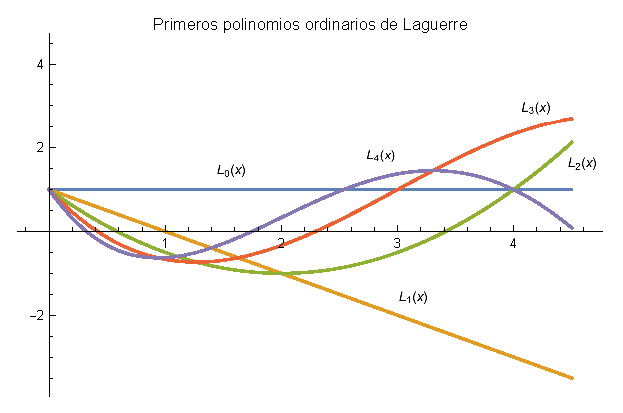
\includegraphics[scale=0.85]{Imagenes/Polinomios_Laguerre_03.eps}
    \caption{Gráfica con los primeros polinomios ordinarios de Legendre $L_{n}(x)$.}
    \label{fig:grafica_Laguerre_01}
\end{figure}
\end{frame}

\subsection{Propiedades de \texorpdfstring{$L_{n}(x)$}{L n (x)}}

\begin{frame}
\frametitle{Utilidad de los $L_{n}(x)$}
Los polinomios de Laguerre y las funciones derivadas de ellos son importantes en el análisis del comportamiento de algunos sistemas físicos en la mecánica cuántica, como lo hemos revisado en los materiales de trabajo previos.
\end{frame}
\begin{frame}
\frametitle{Revisando las propiedades}
Notarán que el orden en que se revisan las propiedades y características es diferente al que se presentó con los polinomios de Legendre, \pause no hay como tal, un orden preciso de revisión, pero si es importante presentar todas las propiedades.
\end{frame}

\subsection{Fórmula de Rodrigues}

\begin{frame}
\frametitle{La expresión}
Los polinomios de Laguerre puede expresarse en términos de la fórmula de Rodrigues, dada por:
\pause
\begin{align}
L_{n} (x) = \dfrac{e^{x}}{n!} \, \dv[n]{x} \left( x^{n} \, e^{-x} \right)
\label{eq:ecuacion_18_112}
\end{align}
\end{frame}
\begin{frame}
\frametitle{De la demostración}
La cual puede demostrarse directamente calculando la enésima derivada usando explícitamente el teorema de Leibnitz y comparando el resultado con la ec. (\ref{eq:ecuacion_18_111}):
\end{frame}
\begin{frame}
\frametitle{Evaluando la derivada}
Evaluando la enésima derivada en la ec. (\ref{eq:ecuacion_18_112}) con el teorema de Leibnitz, se tiene que:
\pause
\begin{eqnarray*}
\begin{aligned}
L_{n}(x) &= \dfrac{e^{x}}{n!} \nsum_{r=0}^{n} \binom{n}{r} \, \dv[r]{x^{n}}{x} \, \dv[n-r]{e^{-x}}{x} = \\[0.5em] \pause
&= \dfrac{e^{x}}{n!} \nsum_{r=0}^{n}  \dfrac{n!}{r! \, (n - r)!} \, \dfrac{n!}{(n - r)!} \, x^{n-r} \, (-1)^{n-r} \, e^{-x} = \\[0.5em] \pause
&= \nsum_{r=0}^{n} (-1)^{n-1} \, \dfrac{n!}{r! \, (n - r)! \, (n - r)!} \, x^{n-r}
\end{aligned}
\end{eqnarray*}
\end{frame}
\begin{frame}
\frametitle{Renombrando índices}
Al renombrar la suma usando el índice $m = n - r$, se llega a:
\pause
\begin{align*}
L_{n}(x) = \nsum_{m=0}^{n} (-1)^{m} \, \dfrac{n!}{(m!)^{2} \, (n - m)!} \, x^{m}
\end{align*}
que es la expresión (\ref{eq:ecuacion_18_111}) para el polinomio de Laguerre de orden $n$.
\end{frame}

\subsection{Ortogonalidad mutua}

\begin{frame}
\frametitle{De la ortogonalidad}
Un resultado que se revisó en el Tema 3, sabemos que la ecuación de Laguerre se podría poner en forma de Sturm Liouville con:
\pause
\begin{eqnarray*}
\begin{aligned}
p &= x \, e^{-x} \\[0.5em] \pause
q &= 0 \\[0.5em] \pause
\lambda &= \nu \\[0.5em] \pause
\omega &= e^{-x}
\end{aligned}
\end{eqnarray*}
y su intervalo natural es entonces $[0, \infty]$.
\end{frame}
\begin{frame}
\frametitle{Ortogonalidad}
Dado que los polinomios de Laguerre $L_{n} (x)$ son soluciones de la ED \pause y son regulares en los puntos extremos, deben ser mutuamente ortogonales en este intervalo con respecto a la función de peso $\omega = e^{-x}$
\end{frame}
\begin{frame}
\frametitle{Ortogonalidad}
Es decir:
\pause
\begin{align*}
\scaleint{6ex}_{\bs 0}^{\infty} L_{n}(x) \, L_{k} (x) \, e^{-x} \dd{x} = 0 \hspace{0.5cm} \text{si } n \neq k
\end{align*}
Este resultado se puede demostrar usando directamente la fórmula de Rodrigues - ec. (\ref{eq:ecuacion_18_112}).
\end{frame}
\begin{frame}
\frametitle{De la normalización}
De hecho, la normalización, cuando $k = n$, es más fácil de demostrar usando este método, tendremos entonces que:
\pause
\begin{align}
I \equiv \scaleint{6ex}_{\bs 0}^{\infty} L_{n} (x) \, L_{n} (x) \, e^{-x} \dd{x} = 1
\label{eq:ecuacion_18_113}
\end{align}
\end{frame}
\begin{frame}
\frametitle{Usando las propiedades}
Usando la fórmula de Rodrigues, podemos escribir:
\pause
\begin{eqnarray*}
\begin{aligned}
I &= \dfrac{1}{n!} \, \scaleint{6ex}_{\bs 0}^{\infty} L_{n}(x) \, \dv[n]{x} \left( x^{n} \, e^{-x} \right) \dd{x} = \\[0.5em] \pause
&= \dfrac{(-1)^{n}}{n!} \scaleint{6ex}_{\bs 0}^{\infty} \dv[n]{L_{n}}{x} \, x^{n} \, e^{-x} \dd{x}
\end{aligned}
\end{eqnarray*}
\pause
en la segunda igualdad se ha integrado por partes $n$ veces y con el hecho de que los términos en los extremos se anulan.
\end{frame}
\begin{frame}
\frametitle{Los términos que permanecen}
Cuando el término $\dv*[n]{L_{n}}{x}$ se evalúa usando la ec. (\ref{eq:ecuacion_18_111}), solo la derivada de $m = n$ términos sobreviven y tienen el valor:
\pause
\begin{align*}
\dfrac{(-1)^{n} \, n! \, n!}{(n!)^{2} \, 0!} = (-1)^{n}
\end{align*}
\end{frame}
\begin{frame}
\frametitle{Resultado}
Entonces tenemos que:
\pause
\begin{align*}
I = \dfrac{1}{n!} \scaleint{6ex}_{\bs 0}^{\infty} x^{n} \, e^{-x} \dd{x} = 1
\end{align*}
en la segunda igualdad, se ha utilizado la ec. (\ref{eq:ecuacion_18_113}) definiendo la función Gamma.
\end{frame}

\subsection{Expansión de funciones}

\begin{frame}
\frametitle{Expandiendo funciones}
Las condiciones de normalización y ortogonalidad anteriores nos permiten expandir cualquier función $f (x)$ (razonable) en el intervalo $0 \leq x < \infty$ en una serie de la forma:
\pause
\begin{align*}
f (x) = \nsum_{n=0}^{\infty} a_{n} \, L_{n} (x)
\end{align*}
\pause
en la cual, los coeficientes $a_{n}$ están dado por:
\pause
\begin{align*}
a_{n} = \scaleint{6ex}_{\bs 0}^{\infty} f(x) \, L_{n}(x) \, e^{-x} \dd{x}
\end{align*}
\end{frame}
\begin{frame}
\frametitle{Funciones ortonormales}
Observamos que a veces es conveniente definir las \textocolor{carmine}{funciones de Laguerre ortonormales} $\phi_{n} (x) = e^{-x/2} \, L_{n} (x)$, que también pueden usarse para producir una expansión en series de una función en el intervalo $0 \leq x < \infty$.
\end{frame}

\subsection{Función generatriz}

\begin{frame}
\frametitle{Expresión para la función}
La función generatriz para los polinomios de Laguerre está dada por:
\pause
\begin{align}
G (x, h) = \dfrac{e^{-xh/(1-h)}}{1- h} = \nsum_{n=0}^{\infty} L_{n} (x) \, h^{n}
\label{eq:ecuacion_18_114}
\end{align}
\end{frame}

\subsection{Relaciones de recurrencia}\label{sec:subsub_relaciones_recurrencia}

\begin{frame}
\frametitle{Obteniendo las relaciones}
Podemos probar este resultado diferenciando la función generatriz con respecto a $x$ y $h$, respectivamente, \pause para obtener relaciones de recurrencia para los polinomios de Laguerre, que luego pueden combinarse para mostrar que las funciones $L_{n} (x)$ en la ec. (\ref{eq:ecuacion_18_114}) satisfacen efectivamente la fórmula de Laguerre.
\end{frame}
\begin{frame}
\frametitle{Diferenciación con respecto a $h$}
Diferenciando la función generatriz (\ref{eq:ecuacion_18_114}) con respecto a $h$, se tiene que:
\pause
\begin{align*}
\pdv{G}{h} = \dfrac{(1 - x -h) \, e^{-xh/(1-h)}}{(1- h )^{3}} = \nsum n \, L_{n} \, h^{n-1}
\end{align*}
\end{frame}
\begin{frame}
\frametitle{Avanzando en la operación}
Por lo que podemos escribir:
\pause
\begin{align*}
(1 - x - h) \nsum L_{n} \, h^{n} = (1 - h)^{2} \nsum n \, L_{n} \, h^{n-1}
\end{align*}
\end{frame}
\begin{frame}
\frametitle{Igualando coeficientes}
Que al igualar los coeficientes de $h^{n}$ en cada lado de la igualdad, obtenemos:
\pause
\begin{align*}
(1 - x) \, L_{n} - L_{n-1} &= (n + 1) \, L_{n+1} - 2 \, n \, L_{n} + \\[0.5em]
&+ (n + 1) \, L_{n+1}
\end{align*}
\end{frame}
\begin{frame}
\frametitle{Manejando la expresión}
Que simplificamos y ordenamos los términos para establecer una relación de recurrencia:
\pause
\begin{align}
\begin{aligned}[b]
(n + 1) \, L_{n+1} (x) &= (2 \, n + 1 - x) \, L_{n}(x) + \\[0.5em]
&- n \, L_{n-1} (x)
\end{aligned}
\label{eq:ecuacion_18_115}
\end{align}
lo que nos permite encontrar el polinomio de Laguerre de orden $(n+1)$ a partir de los polinomios de orden $n$ y $n+1$.
\end{frame}
\begin{frame}
\frametitle{Diferenciación con respecto a $x$}
Al diferenciar la función generatriz con respecto a $x$, tendremos lo siguiente:
\pause
\begin{align*}
\pdv{G}{x} = \dfrac{h \, e^{-xh/(1-h)}}{(1 - h)^{2}} = \nsum n \, \pderivada{L}_{n} \, h^{n}
\end{align*}
\end{frame}
\begin{frame}
\frametitle{Resultado}
Lo que nos conduce a:
\pause
\begin{align*}
- h \nsum L_{n} \, h^{n} =  (1 - h) \, \nsum \pderivada{L}_{n} \, h^{n}
\end{align*}
\pause
que al igualar los coeficientes de $h^{n}$ en cada lado de la igualdad, llegamos a:
\pause
\begin{align}
- L_{n-1} (x) = \pderivada{L}_{n} - \pderivada{L}_{n-1}
\label{eq:ecuacion_18_116}
\end{align}
\end{frame}
\begin{frame}
\frametitle{Combinando resultados}
Haciendo una combinación de los resultados obtenidos en las ecs. (\ref{eq:ecuacion_18_115}) y (\ref{eq:ecuacion_18_116}), es posible obtener una tercera relación de recurrencia:
\pause
\begin{align}
x \, \pderivada{L}_{n} (x) = n \, L_{n} (x) - n \, L_{n-1} (x)
\label{eq:ecuacion_18_117}
\end{align}
\end{frame}

\section{Funciones asociadas de Laguerre}
\frame[allowframebreaks]{\tableofcontents[currentsection, hideothersubsections]}
\subsection{La ED de partida}

\begin{frame}
\frametitle{La ED inicial}
El ecuación diferencial de Laguerre es de la forma:
\pause
\begin{align}
x \, \sderivada{y} + (m +  1 - x) \, \pderivada{y} + n \, y = 0
\label{eq:ecuacion_18_118}
\end{align}
tiene una singularidad regular en $x = 0$ y una singularidad esencial en $x = \infty$.
\end{frame}
\begin{frame}
\frametitle{Acotando valores}
Restringimos nuestra atención a la situación en la que los parámetros $n$ y $m$ son números enteros no negativos, como es el caso de casi todos los problemas físicos.
\end{frame}
\begin{frame}
\frametitle{Naturaleza de la ED}
La ecuación de Laguerre asociada ocurre con mayor frecuencia en aplicaciones de la mecánica cuántica.
\\
\bigskip
\pause
Cualquier solución de la ec. (\ref{eq:ecuacion_18_118}) se denomina \textocolor{byzantine}{función asociada de Laguerre}.
\end{frame}
\begin{frame}
\frametitle{Soluciones a la ED}
Las soluciones de (\ref{eq:ecuacion_18_118}) para números enteros no negativos $n$ y $m$ están dadas por los polinomios de asociados de Laguerre:
\pause
\begin{align}
L_{n}^{m} (x) = (-1)^{m} \dv[m]{x} L_{n+m} (x) \hspace{1.5cm} m \leq n
\label{eq:ecuacion_18_119}
\end{align}
donde $L_{n} (x)$ son los polinomios ordinarios de Laguerre.
\end{frame}
\begin{frame}
\frametitle{Valor de un polinomio}
En particular debemos de revisar que $L_{n}^{0} (x) = L_{n}(x)$, \pause ya hemos comentado que $L_{n} (x)$ es un polinomio de orden $n$ por lo que $L_{n}^{m} (x)$ también lo es.
\end{frame}
\begin{frame}
\frametitle{Expresiones de los polinomios}
Los primeros polinomios asociados de Laguerre se calculan fácilmente a partir de la ec. (\ref{eq:ecuacion_18_119}):
\pause
\begin{eqnarray*}
\begin{aligned}
L_{0}^{m} (x) &= 1 \\[0.5em] \pause
L_{1}^{m} (x) &= -x + m + 1 \\[0.5em] \pause
2! \, L_{2}^{m} (x) &= x^{2} - 2 (m + 2) \, x + (m + 1)(m + 2) \\[0.5em]
\vdots
\end{aligned}
\end{eqnarray*}
\end{frame}
\begin{frame}[plain]
\begin{figure}[H]
    \centering
    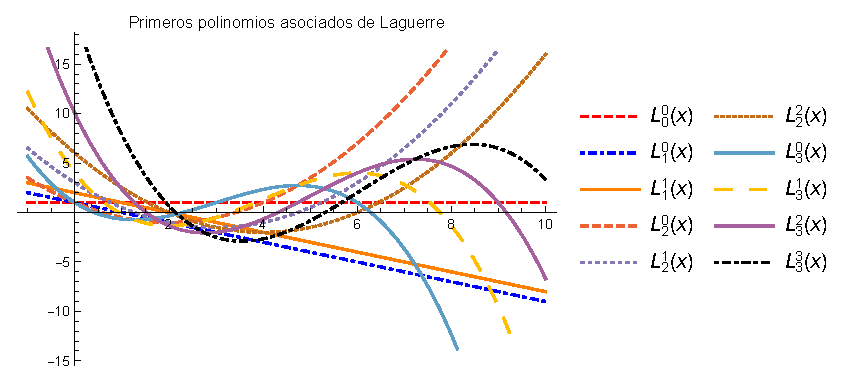
\includegraphics[scale=0.75]{Imagenes/Polinomios_Laguerre_04.eps}
    % \caption{Primeros polinomios asociados de Laguerre.}
    % \label{fig:grafica_Laguerre_02}
\end{figure}
\end{frame}
\begin{frame}
\frametitle{Expresión alterna}
De hecho, en el caso general, se puede demostrar directamente, a partir de la definición (\ref{eq:ecuacion_18_119}) y la ec. (\ref{eq:ecuacion_18_111}) para los polinomios ordinarios de Laguerre, que:
\pause
\begin{align}
L_{n}^{m} (x) = \nsum_{k=0}^{n} (-1)^{k} \, \dfrac{(n + m)!}{k! \, (n - k)! \, (k + m)!} \, x^{k}
\label{eq:ecuacion_18_120}
\end{align}
\end{frame}

\subsection{Propiedades Asociados de Laguerre}

\begin{frame}
\frametitle{Relación con los ordinarios de Laguerre}
Las propiedades de los polinomios asociados de Laguerre se derivan directamente de las de los polinomios ordinarios de Laguerre a través de la definición ec. (\ref{eq:ecuacion_18_119}).
\\
\bigskip
\pause
Por lo tanto, aquí sólo describiremos brevemente los resultados más útiles.
\end{frame}

\subsection{Fórmula de Rodrigues}

\begin{frame}
\frametitle{La fórmula de Rodrigues}
La fórmula de Rodrigues de los polinomios asociados de Laguerre está dada por la expresión:
\pause
\begin{align}
L_{n}^{m} (x) = \dfrac{e^{x} \, x^{-m}}{n!} \, \dv[n]{x} \left( x^{n+m} \, e^{-x} \right)
\label{eq:ecuacion_18_121}
\end{align}
Que se puede demostrar al evaluar la enésima derivada usando el teorema de Leibnitz.
\end{frame}

\subsection{Ortogonalidad mutua}

\begin{frame}
\frametitle{Condición de ortogonalidad}
Del Tema 3 del curso sabemos que la ED asociada de Laguerre podría transformarse en una ecuación de tipo Sturm Liouville con:
\pause
\begin{eqnarray*}
\begin{aligned}
p &= x^{m+1} \, e^{-x} \\ \pause
q &= 0 \\ \pause
\lambda &= n \\ \pause
\omega =& x^{m} \, e^{-x}
\end{aligned}
\end{eqnarray*}
y su intervalo natural es entonces $[0, \infty]$.
\end{frame}
\begin{frame}
\frametitle{Condición de ortogonalidad}
Dado que los polinomios asociados de Laguerre $L_{m}^{n} (x)$ son soluciones de la ecuación y son regulares en los puntos extremos, \pause aquellos con el mismo $m$ pero valores diferentes del valor propio $\lambda = n$ deben ser mutuamente ortogonales en este intervalo con respecto a la función de peso $\omega = x^{m} \, e^{-x}$
\end{frame}
\begin{frame}
\frametitle{Condición de ortogonalidad}
Es decir:
\pause
\begin{align*}
\scaleint{6ex}_{\bs 0}^{\infty} L_{n}^{m} (x) \, L_{k}^{m} (x) \, x^{m} \, e^{-x} \dd{x} = 0 \hspace{1.5cm} \mbox{si } n \neq k
\end{align*}
\end{frame}
\begin{frame}
\frametitle{Demostrando la propiedad}
Este resultado también se puede demostrar utilizando la fórmula de Rodrigues (\ref{eq:ecuacion_18_121}), al igual que la condición de normalización cuando $k = n$:
\pause
\begin{align}
I \equiv \scaleint{6ex}_{\bs 0}^{\infty} L_{n}^{m} (x) \, L_{n}^{m} (x) \, x^{m} \, e^{-x} \dd{x} =\dfrac{(n + m)!}{n!}
\label{eq:ecuacion_18_122}
\end{align}
\end{frame}
\begin{frame}
\frametitle{Demostrando la propiedad}
Usando la fórmula de Rodrigues (\ref{eq:ecuacion_18_121}), podemos escribir:
\pause
\begin{eqnarray*}
\begin{aligned}
I &= \dfrac{1}{n!} \scaleint{6ex}_{\bs 0}^{\infty} L_{n}^{m} \, \dv[n]{x} \left( x^{n+m} \, e^{-x} \right) \dd{x} = \\[0.5em] \pause 
&= \dfrac{(-1)^{n}}{n!} \scaleint{6ex}_{\bs 0}^{\infty} \dv[n]{L_{n}^{m}}{x} \, x^{n+m} \, e^{-x} \dd{x}
\end{aligned}
\end{eqnarray*}
\end{frame}
\begin{frame}
\frametitle{Demostrando la propiedad}
En la segunda igualdad se ha integrado por partes $n$ veces y se ha utilizado el hecho de que los términos en los extremos se anulan.
\\
\bigskip
\pause
De la ec. (\ref{eq:ecuacion_18_120}) tenemos que:
\pause
\begin{align*}
I = \dfrac{1}{n!} \scaleint{6ex}_{\bs 0}^{\infty} x^{n+m} \, e^{-x} \dd{x} = \dfrac{(n + m)!}{n!}
\end{align*}
en la segunda igualdad, se ha ocupado la definición de la función Gamma.
\end{frame}

\subsection{Expansión de funciones}

\begin{frame}
\frametitle{Expresando funciones}
Dada las condiciones de ortogonalidad y normalización, es posible expandir cualquier función $f (x)$ (razonable) en el intervalo $0 \leq x < \infty$ en una serie de la forma:
\pause
\begin{align*}
f (x) = \nsum_{n=0}^{\infty} a_{n} \, L_{n}^{m} (x)
\end{align*}
\end{frame}
\begin{frame}
\frametitle{Los coeficientes de la expansión}
En la cual, los coeficientes $a_{n}$ están dado por la expresión:
\pause
\begin{align*}
a_{n} = \dfrac{n!}{(n + m)!} \scaleint{6ex}_{\bs 0}^{\infty} f(x) \, L_{n}^{m}(x) \, x^{m} \, e^{-x} \dd{x}
\end{align*}
\end{frame}
\begin{frame}
\frametitle{Funciones ortonormales}
Es conveniente conocer que en ocasiones se definen las \textocolor{bole}{funciones ortogonales asociadas de Laguerre}:
\pause
\begin{align*}
\phi_{n}^{m} (x) = x^{m/2} \, e^{-x/2} \, L_{n}^{m} (x)
\end{align*}
que también se puede utilizar para producir una expansión en series de una función en el intervalo $0 \leq x < \infty$.
\end{frame}

\subsection{Función generatriz}

\begin{frame}
\frametitle{La función generatriz}
La función generatriz de los polinomios asociados de Laguerre están dados por:
\pause
\begin{align}
G (x, h) = \dfrac{\exp\big[(-x \, h)/(1 - h)\big]}{(1 - h)^{m+1}} = \nsum_{n=0}^{\infty} L_{n}^{m} (x) \, h^{n}
\label{eq:ecuacion_18_123}
\end{align}
\end{frame}
\begin{frame}
\frametitle{De la función generatriz}
Esta expresión se obtiene al diferenciar $m$ veces con respecto a $x$ la función generatriz (\ref{eq:ecuacion_18_114}) de los polinomios ordinarios de Laguerre y ocupando la ec. (\ref{eq:ecuacion_18_119}).
\end{frame}
\begin{frame}
\frametitle{Usando la función generatriz}
Como ejemplo del uso de la función generatriz veamos su manejo para obtener una expresión de $L_{n}^{m}(0)$:
\end{frame}
\begin{frame}
\frametitle{Usando la función generatriz}
Tenemos entonces que:
\pause
\begin{eqnarray*}
\begin{aligned}
&\nsum_{n=0}^{\infty} L_{n}^{m} (0) \, h^{n} = \dfrac{1}{(1 - h)^{m+1}} = \\[0.5em] \pause
&= 1 + (m + 1) \, h + \dfrac{(m + 1)(m + 2)}{2!} \, h^{2} + \ldots + \\[0.5em] \pause
&+ \dfrac{(m + 1)(m + 2) \ldots (m + n)}{n!} \, h^{n} + \ldots  
\end{aligned}
\end{eqnarray*}
en la segunda igualdad, se ha expandido el lado derecho usando el teorema del binomio.
\end{frame}
\begin{frame}
\frametitle{Usando la función generatriz}
Al igualar los coeficientes de $h^{n}$, se obtiene:
\pause
\begin{align*}
L_{n}^{m} (0) = \dfrac{(n + m)!}{n! \, m!}
\end{align*}
\end{frame}

\subsection{Relaciones de recurrencia}

\begin{frame}
\frametitle{De las relaciones de recurrencia}
Las distintas relaciones de recurrencia por los polinomios asociados de Laguerre se obtienen diferenciando la función generadora (\ref{eq:ecuacion_18_123}) con respecto a uno o ambos de $x$ y $h$, \pause o diferenciando con respecto a $x$ las relaciones de recurrencia de los polinomios ordinarios de Laguerre.
\end{frame}
\begin{frame}
\frametitle{Las expresiones}
De las relaciones de recurrencia de los polinomios asociados de Laguerre, se presentan a continuación las más útiles:
\pause
\begin{eqnarray*}
\begin{aligned}
&(n {+} 1) \, L_{n+1}^{m} (x) = (2 n {+} m {+} 1 {-} x) \, L_{n}^{m} (x) {-} (n {+} m) \, L_{n-1}^{m} (x) \\[0.5em]
&x \, \pderivada{(L_{n}^{m})} (x) = n \, L_{n}^{m} (x) - (n {+} m) \, L_{n-1}^{m} (x) \\[0.5em]
&\pderivada{L_{n}^{m}} = - L_{n-1}^{m+1} (x)  \\[0.5em]
&L_{n}^{m} (x) = L_{n}^{m+1} (x) - L_{n-1}^{m+1} (x)  \\[0.5em]
&n \, L_{n}^{m} (x) = (n {+} m) \, L_{n-1}^{m} (x) - x \, L_{n-1}^{m+1} (x) 
\end{aligned}
\end{eqnarray*}
\end{frame}

\section{Teorema del desarrollo}
\frame[allowframebreaks]{\tableofcontents[currentsection, hideothersubsections]}
\subsection{Definición}

\begin{frame}
\frametitle{Definición del teorema}
El teorema del desarrollo nos permite expresar una función cualquiera en términos de una serie infinita incluyendo una función especial:
\pause
\begin{align*}
f (x) = \nsum_{n=0}^{\infty} c_{n} \, \mathbf{F}_{n} (x)
\end{align*}
donde $\mathbf{F}_{n}(x)$ es una función especial que depende de un parámetro $n$.
\end{frame}
\begin{frame}
\frametitle{La base completa de los $L_{n}^{k}(x)$}
Los polinomios asociados de Laguerre forman una base completa:
\begin{align*}
\left\{ \scaleto{L_{n}^{k}(x)}{3ex} \right\}
\end{align*}
\pause
por lo que de acuerdo con el teorema del desarrollo, podemos expresar una función $f (x)$ como una serie infinita del producto de unos coeficientes por los polinomios asociados de Laguerre.
\end{frame}
\begin{frame}
\frametitle{Problema a resolver}
Entonces tendremos que:
\pause
\begin{align*}
\exp(-a \, x) = \nsum_{n=0}^{\infty} c_{n} \, \scaleto{L_{n}^{k}(x)}{3ex}
\end{align*}
Debiendo obtener los respectivos coeficientes $c_{n}$.
\end{frame}

\subsection{Resolviendo el problema}

\begin{frame}
\frametitle{Paso previo a la solución}
Se requiere \enquote{adecuar} la expresión que tenemos para un siguiente paso, en donde se ocuparán algunas de las propiedades de los polinomios asociados de Laguerre.
\pause
\\
\bigskip
Dependiendo de la función especial que esté involucrada, el manejo es diferente, pero la idea es la misma.
\end{frame}
\begin{frame}
\frametitle{Multiplicando por un $1$}
Multiplicamos la función por:
\pause
\begin{align*}
\exp(-x) \, x^{k} \, L_{m}^{k}(x)
\end{align*}
para luego integrar con respecto a $x$ de $0$ a $\infty$:
\pause
\begin{eqnarray*}
\begin{aligned}
\scaleint{6ex}_{\bs 0}^{\infty} \exp(- a \, x) \, \bigg[ \exp(-x) \, x^{k} \, L_{m}^{k}(x) \bigg] \dd{x}
= \\[1em] \pause
\scaleint{6ex}_{\bs 0}^{\infty} \, \nsum_{n=0}^{\infty} c_{n} \, L_{n}^{k}(x) \, \bigg[ \exp(-x) \, x^{k} \, L_{m}^{k}(x) \bigg] \dd{x}
\end{aligned}
\end{eqnarray*}
\end{frame}
\begin{frame}
\frametitle{Acomodamos términos}
Haciendo álgebra:
\pause
\begin{eqnarray*}
\begin{aligned}
\scaleint{6ex}_{\bs 0}^{\infty} \exp( -[ a + 1] \, x) \, x^{k} \, L_{m}^{k}(x) \dd{x}
= \\[1em] \pause
\nsum_{n=0}^{\infty} c_{n} \scaleint{6ex}_{\bs 0}^{\infty} \exp(-x) \, x^{k} \, L_{n}^{k}(x) \, L_{m}^{k}(x) \dd{x}    
\end{aligned}
\end{eqnarray*}
\pause
Usaremos la propiedad de ortogonalidad de los $L_{m}^{k}(x)$.
\end{frame}

\subsection{Usando propiedades}

\begin{frame}
\frametitle{La propiedad de ortogonalidad}
La propiedad de ortogonalidad de los polinomios asociados de Laguerre es:
\pause
\begin{align*}
\scaleint{6ex}_{\bs 0}^{\infty} \exp(-x) \, x^{k} \, L_{n}^{k}(x) \, L_{m}^{k}(x) \dd{x} = \dfrac{(n + k)!}{n!} \, \delta_{mn}
\end{align*}
\end{frame}
\begin{frame}
\frametitle{Lado derecho de la igualdad}
Se tendrá entonces que el lado derecho de la igualdad es:
\begin{eqnarray*}
= \nsum_{n=0}^{\infty} c_{n} \, \dfrac{(n + k)!}{n!} \, \delta_{mn} = \pause c_{n} \, \dfrac{(n + k)!}{n!}
\end{eqnarray*}
\end{frame}
\begin{frame}
\frametitle{Regresando a la igualdad}
Entonces el lado izquierdo de la igualdad es:
\pause
\begin{align*}
\scaleint{6ex}_{\bs 0}^{\infty} \exp( -[ a + 1] \, x) \, x^{k} \, L_{m}^{k}(x) \dd{x} = c_{n} \, \dfrac{(n + k)!}{n!}
\end{align*}
\pause
De donde podemos despejar a los coeficientes $c_{n}$.
\end{frame}
\begin{frame}
\frametitle{Expresión para los coeficientes}
Al separar los $c_{n}$, llegamos a:
\pause
\begin{align*}
c_{n} = \dfrac{n!}{(n+ k)!} \, \scaleint{6ex}_{\bs 0}^{\infty} \exp( -[ a + 1] \, x) \, x^{k} \, L_{m}^{k}(x) \dd{x}
\end{align*}
\pause
Para resolver la integral, tendremos que ocupar otra de las propiedades de los $L_{m}^{k}(x)$.
\end{frame}
\begin{frame}
\frametitle{Uso de la fórmula de Rodrigues}
La expresión que define a la fórmula de Rodrigues para los polinomios asociados de Laguerre es:
\pause
\begin{align*}
\scaleto{L_{m}^{k}(x)}{3ex} = \dfrac{e^{x} \, x^{-k}}{n!} \, \dv[n]{x} \bigg( e^{-x} \, x^{n+k} \bigg)
\end{align*}
\end{frame}
\begin{frame}
\frametitle{Con la fórmula de Rodrigues}
La expresión de los coeficientes pasa a ser:
\pause
\begin{align*}
c_{n} = &\dfrac{n!}{(n+ k)!} \, \scaleint{6ex}_{\bs 0}^{\infty} \exp( -[ a + 1] \, x) \, x^{k} \, \times \\[1em]  
&\times \bigg[ \dfrac{e^{x} \, x^{-k}}{n!} \, \dv[n]{x} \bigg( e^{-x} \, x^{n+k} \bigg) \bigg] \dd{x}
\end{align*}
\pause
Organizamos y reducimos los términos de la expresión.
\end{frame}
\begin{frame}
\frametitle{Expresión simplificada}
Se tiene que:
\pause
\begin{align*}
c_{n} = &\dfrac{ \Cancel[red]{n}!}{\Cancel[red]{n!} (n+ k)!} \, \scaleint{6ex}_{\bs 0}^{\infty} \exp( -[ a \, \Cancel[red]{+ 1} \Cancel[red]{- 1}] \, x) \, x^{\Cancel[red]{k}-\Cancel[red]{k}} \, \times \\[1em]  
&\times \bigg[ \dv[n]{x} \bigg( e^{-x} \, x^{n+k} \bigg) \bigg] \dd{x}
\end{align*}
\end{frame}
\begin{frame}
\frametitle{Expresión simplificada}
La expresión para los coeficientes es:
\pause
\begin{align*}
c_{n} = &\dfrac{ 1}{(n+ k)!} \, \scaleint{6ex}_{\bs 0}^{\infty} \exp( - a \, x) \, \dv[n]{x} \bigg( e^{-x} \, x^{n+k} \bigg) \dd{x}
\end{align*}
Tenemos que el integrando involucra la derivada de orden $n$.
\end{frame}
\begin{frame}
\frametitle{Resolviendo la integral}
La integral se resuelve por partes, donde:
\pause
\begin{align*}
u = \exp(-a \, x) \hspace{1cm} \dd{u} = - a \, \exp(-a \, x) \dd{x} 
\end{align*}
\pause
\begin{align*}
\dd{v} = \dv[n]{x} \bigg[ e^{-x} \, x^{n+k} \bigg] \hspace{1cm} v = \dv[n-1]{x} \bigg[ e^{-x} \, x^{n+k+1} \bigg]
\end{align*}
\pause
Usaremos de nuevo la fórmula de Rodrigues para expresar el valor de $v$.
\end{frame}
\begin{frame}
\frametitle{Un resultado oportuno}
El valor de $v$ será entonces:
\pause
\begin{align*}
v = (n - 1)! \, e^{-x} \, x^{k+1} \, \scaleto{L_{n-1}^{k+1}(x)}{3ex}
\end{align*}
\pause
que habrá que ocupar en el cálculo de los exponentes $c_{m}$:
\end{frame}
\begin{frame}
\frametitle{Resultado de la integración por partes}
Se tiene que:
\pause
\begin{align*}
c_{n} &= \dfrac{ 1}{(n {+} k)!} \, \bigg[ \exp(-[a {+} 1] \, x) \, x^{k+1} \, (n {-} 1)! \times \\[0.5em]
&\times L_{n-1}^{k+1}(x) \bigg] \bigg\vert_{0}^{\infty} + \\[1em]
&+ a \, \scaleint{6ex}_{\bs 0}^{\infty} \exp( - a \, x) \, \dv[n-1]{x} \bigg( e^{-x} \, x^{n+k} \bigg) \dd{x}
\end{align*}
\pause
Estudiemos el término entre corchetes.
\end{frame}
\begin{frame}
\frametitle{Término entre corchetes}
\begin{align*}
\bigg[ \exp(-[a + 1] \, x) \, x^{k+1} \, (n - 1)! L_{n-1}^{k+1}(x) \bigg] \bigg\vert_{0}^{\infty}
\end{align*}
\pause
Cuando $x \to \infty$, todo el corchete de anula, debido a que el término $\exp(-[a + 1] \, x) \to 0$, \pause el corchete se cancela.
\\
\bigskip
\pause
Ahora que cuando $x \to 0$, todo el corchete también se anula, debido a que el término $x^{k+1} = 0$, el corchete también se cancela.
\end{frame}
\begin{frame}
\frametitle{Continuando con el cálculo de los $c_{n}$}
Entonces se tiene que los coeficientes son:
\pause
\begin{align*}
c_{n} = a \, \scaleint{6ex}_{\bs 0}^{\infty} \exp( - a \, x) \, \dv[n-1]{x} \bigg( e^{-x} \, x^{n+k} \bigg) \dd{x}
\end{align*}
\pause
Por lo que nuevamente integramos por partes,
donde:
\pause
\begin{align*}
u = \exp(-a \, x) \hspace{1cm} \dd{u} = - a \, \exp(-a \, x) \dd{x} 
\end{align*}
\pause
\begin{align*}
\dd{v} = \dv[n-1]{x} \bigg[ e^{-x} \, x^{n+k} \bigg] \hspace{1cm} v = \dv[n-2]{x} \bigg[ e^{-x} \, x^{n+k} \bigg]
\end{align*}
\end{frame}
\begin{frame}
\frametitle{Ocupando de nuevo la fórmula de Rodrigues}
De la expresión de $v$, con la fórmula de Rodrigues, tenemos que:
\pause
\begin{align*}
v = (n - 2)! \, e^{-x} \, x^{k+2} \, \scaleto{L_{n-2}^{k+2}(x)}{3ex}
\end{align*}
\pause
Para ocuparlo en la expresión de los $c_{n}$.
\end{frame}
\begin{frame}
\frametitle{Integrando por partes de nuevo}
Resulta ser que:
\pause
\begin{align*}
c_{n} &= \dfrac{a}{(n ^{+} k)!} \, \bigg[ \exp(-[a ^{+} 1] \, x) \, x^{k+2} \, (n ^{+} 2)! \times \\[0.5em]
&\times  L_{n-2}^{k+2}(x) \bigg] \bigg\vert_{0}^{\infty} + \\[1em]
&+ a \, \scaleint{6ex}_{\bs 0}^{\infty} \exp( - a \, x) \, \dv[n-2]{x} \bigg( e^{-x} \, x^{n+k} \bigg) \dd{x}
\end{align*}
\pause
Otra vez estudiemos el término entre corchetes.
\end{frame}
\begin{frame}
\frametitle{Término entre corchetes}
\begin{align*}
\bigg[ \exp(-[a + 1] \, x) \, x^{k+2} \, (n - 2)! \scaleto{L_{n-2}^{k+2}(x)}{3ex} \bigg] \bigg\vert_{0}^{\infty}
\end{align*}
\pause
Cuando $x \to \infty$, el término entre corchetes se anula, debido a que el término $\exp(-[a + 1] \, x) \to 0$
\\
\bigskip
\pause
Ahora que cuando $x \to 0$, el término $x^{k+2} \to  0$, entonces el corchete también se anula.
\end{frame}    
\begin{frame}
\frametitle{Resultado de la segunda integración}
Entonces se tiene que los coeficientes ahora son:
\pause
\begin{align*}
c_{n} = \dfrac{a}{(n + k)!} \, \scaleint{6ex}_{\bs 0}^{\infty} \exp( - a \, x) \, \dv[n-2]{x} \bigg( e^{-x} \, x^{n+k} \bigg) \dd{x}
\end{align*}
\pause
Seguimos resolviendo esta integral por partes $n - 2$ veces, para así obtener:
\end{frame}
\begin{frame}
\frametitle{Resultado luego de integrar $m-2$ veces}
Llegamos al resultado:
\pause
\begin{eqnarray*}
\begin{aligned}
c_{n} &= \dfrac{a^{n}}{(n + k)!} \, \scaleint{6ex}_{\bs 0}^{\infty} \exp( - a \, x) \, \exp(-x) \, x^{n+k} \dd{x} = \\[1em] \pause
&= \dfrac{a^{n}}{(n + k)!} \, \scaleint{6ex}_{\bs 0}^{\infty} \exp(-[a + 1] \, x) \, x^{n+k} \dd{x}
\end{aligned}
\end{eqnarray*}
\pause
Para resolver esta integral haremos un cambio de variable.
\end{frame}
\begin{frame}
\frametitle{Cambio de variable}
Hacemos el cambio de variable: $x = t / (a + 1)$, por lo que:
\pause
\begin{eqnarray*}
\begin{aligned}
\dd{x} &= \dfrac{\dd{t}}{(a + 1)} \\[1em] \pause
\exp([-[a + 1] x]) &= \exp(-t) \\[1em] \pause
x^{n+k} &= \dfrac{t^{n+k}}{(a + 1)^{n+k}}
\end{aligned}
\end{eqnarray*}
\end{frame}
\begin{frame}
\frametitle{Cambio de variable}
Así la integral se transforma en:
\pause
\begin{align*}
c_{n} = \dfrac{a^{n}}{(n + k)! (a + 1)^{n+k+1}} \, \scaleint{6ex}_{\bs 0}^{\infty} e^{-t} \, t^{n+k} \dd{t}
\end{align*}
\pause
del integrando reconocemos a la función Gamma, es decir:
\pause
\begin{align*}
\scaleint{6ex}_{\bs 0}^{\infty} e^{-t} \, t^{n+k} \dd{t} = (n + k)!
\end{align*}
\end{frame}
\begin{frame}
\frametitle{Simplificando la expresión}
Tendremos entonces que:
\pause
\begin{eqnarray*}
\begin{aligned}
c_{n} &= \dfrac{a^{n} \, \Cancel[blue]{(n + k)!}}{\Cancel[blue]{(n + k)!} \, (a + 1)^{n+k+1}} = \\[1em] \pause
&= \dfrac{1}{(a + 1)^{1+k}} \, \left( \dfrac{a}{a + 1} \right)^{n}
\end{aligned}
\end{eqnarray*}
\end{frame}

\subsection{Conclusión}

\begin{frame}
\frametitle{Resultado final}
Al haber definido los coeficientes $c_{n}$, concluimos que mediante el teorema del desarrollo, en la base $\left\{ \scaleto{L_{n}^{k}(x)}{3ex}\right\}$  con $k$ fijo, variando $n$ desde $0$ hasta infinito, la función: 
\begin{align*}
\exp(-a \, x) = \nsum_{n=0}^{\infty} c_{n} \, \scaleto{L_{n}^{k} (x)}{3ex}
\end{align*}
\end{frame}
\begin{frame}
\frametitle{Resultado final}
Se expresa como:
\pause
\begin{align*}
\exp(-a \, x) = \dfrac{1}{(1+a)^{1+k}} \nsum_{n=0}^{\infty} \left( \dfrac{a}{1 + a} \right)^{n} \, \scaleto{L_{n}^{k} (x)}{3ex} \qed
\end{align*}    
\end{frame}

\section{El átomo de hidrógeno}
\frame{\tableofcontents[currentsection, hideothersubsections]}
\subsection{La solución completa}

\begin{frame}
\frametitle{Regresamos al átomo de hidrógeno}
Como ya tenemos las soluciones para la parte radial y angular del átomo de hidrógeno, presentaremos la solución completa al problema con el que iniciamos el Tema.
\end{frame}
\begin{frame}
\frametitle{Funciones de onda normalizadas}
Las funciones de onda normalizadas para el hidrógeno son:
\pause
\begin{align}
\begin{aligned}
\psi_{n \ell m} &= \sqrt{\left(\dfrac{2}{n \, a} \right)^{3} \dfrac{(n - \ell - 1)}{2 \, n[(n + \ell)!]^{3}}} e^{-r/na} \times \\[0.5em]
&\times \left( \dfrac{2 \, r}{n \, a} \right)^{\ell} \; L_{n - \ell -1}^{2 \ell + 1} \left( \dfrac{2 \, r}{n \, a} \right) Y_{\ell}^{m} \, (\theta, \phi)
\end{aligned}
\label{eq:ecuacion_04_89}
\end{align}
\end{frame}
\begin{frame}
\frametitle{Expresión complicada}
No se miran muy agradables, pero no se quejan, este es uno de los muy pocos sistemas realistas que se puede resolver del todo, de forma exacta.
\end{frame}
\begin{frame}
\frametitle{Ortogonalidad de las soluciones}
Son mutuamente ortogonales:
\pause
\begin{align}
\scaleint{6ex} \psi_{n \ell m}^{*} \psi_{\pderivada{n} \pderivada{\ell} \pderivada{m}} \, r^{2} \, \sin \theta \dd{r} \dd{\theta} \dd{\phi} =  \delta_{n \pderivada{n}} \delta_{\ell \pderivada{\ell}} \delta_{m \pderivada{m}}
\label{eq:ecuacion_04_90}
\end{align}
\end{frame}
\begin{frame}
\frametitle{De la ortogonalidad}
Esto se debe a la ortogonalidad de los armónicos esféricos y (para $n \neq n$) de que son las eigenfunciones de $H$ con distinto eigenvalor.
\end{frame}
\begin{frame}
\frametitle{Entendiendo la solución}
Visualizar como tal las funciones de onda del hidrógeno no es fácil, \pause a los químicos les agrada usar \textocolor{armygreen}{gráficas de densidad}, en las cuales el nivel de brillo de la nube es proporcional a $\abs{\Psi}^{2}$, como se puede ver en la figura\footnote{Tomada con licencia de: \url{https://commons.wikimedia.org/wiki/File:Hydrogen_Density_Plots.png}}:
\end{frame}
\begin{frame}[plain]
\begin{figure}[H]
    \centering
    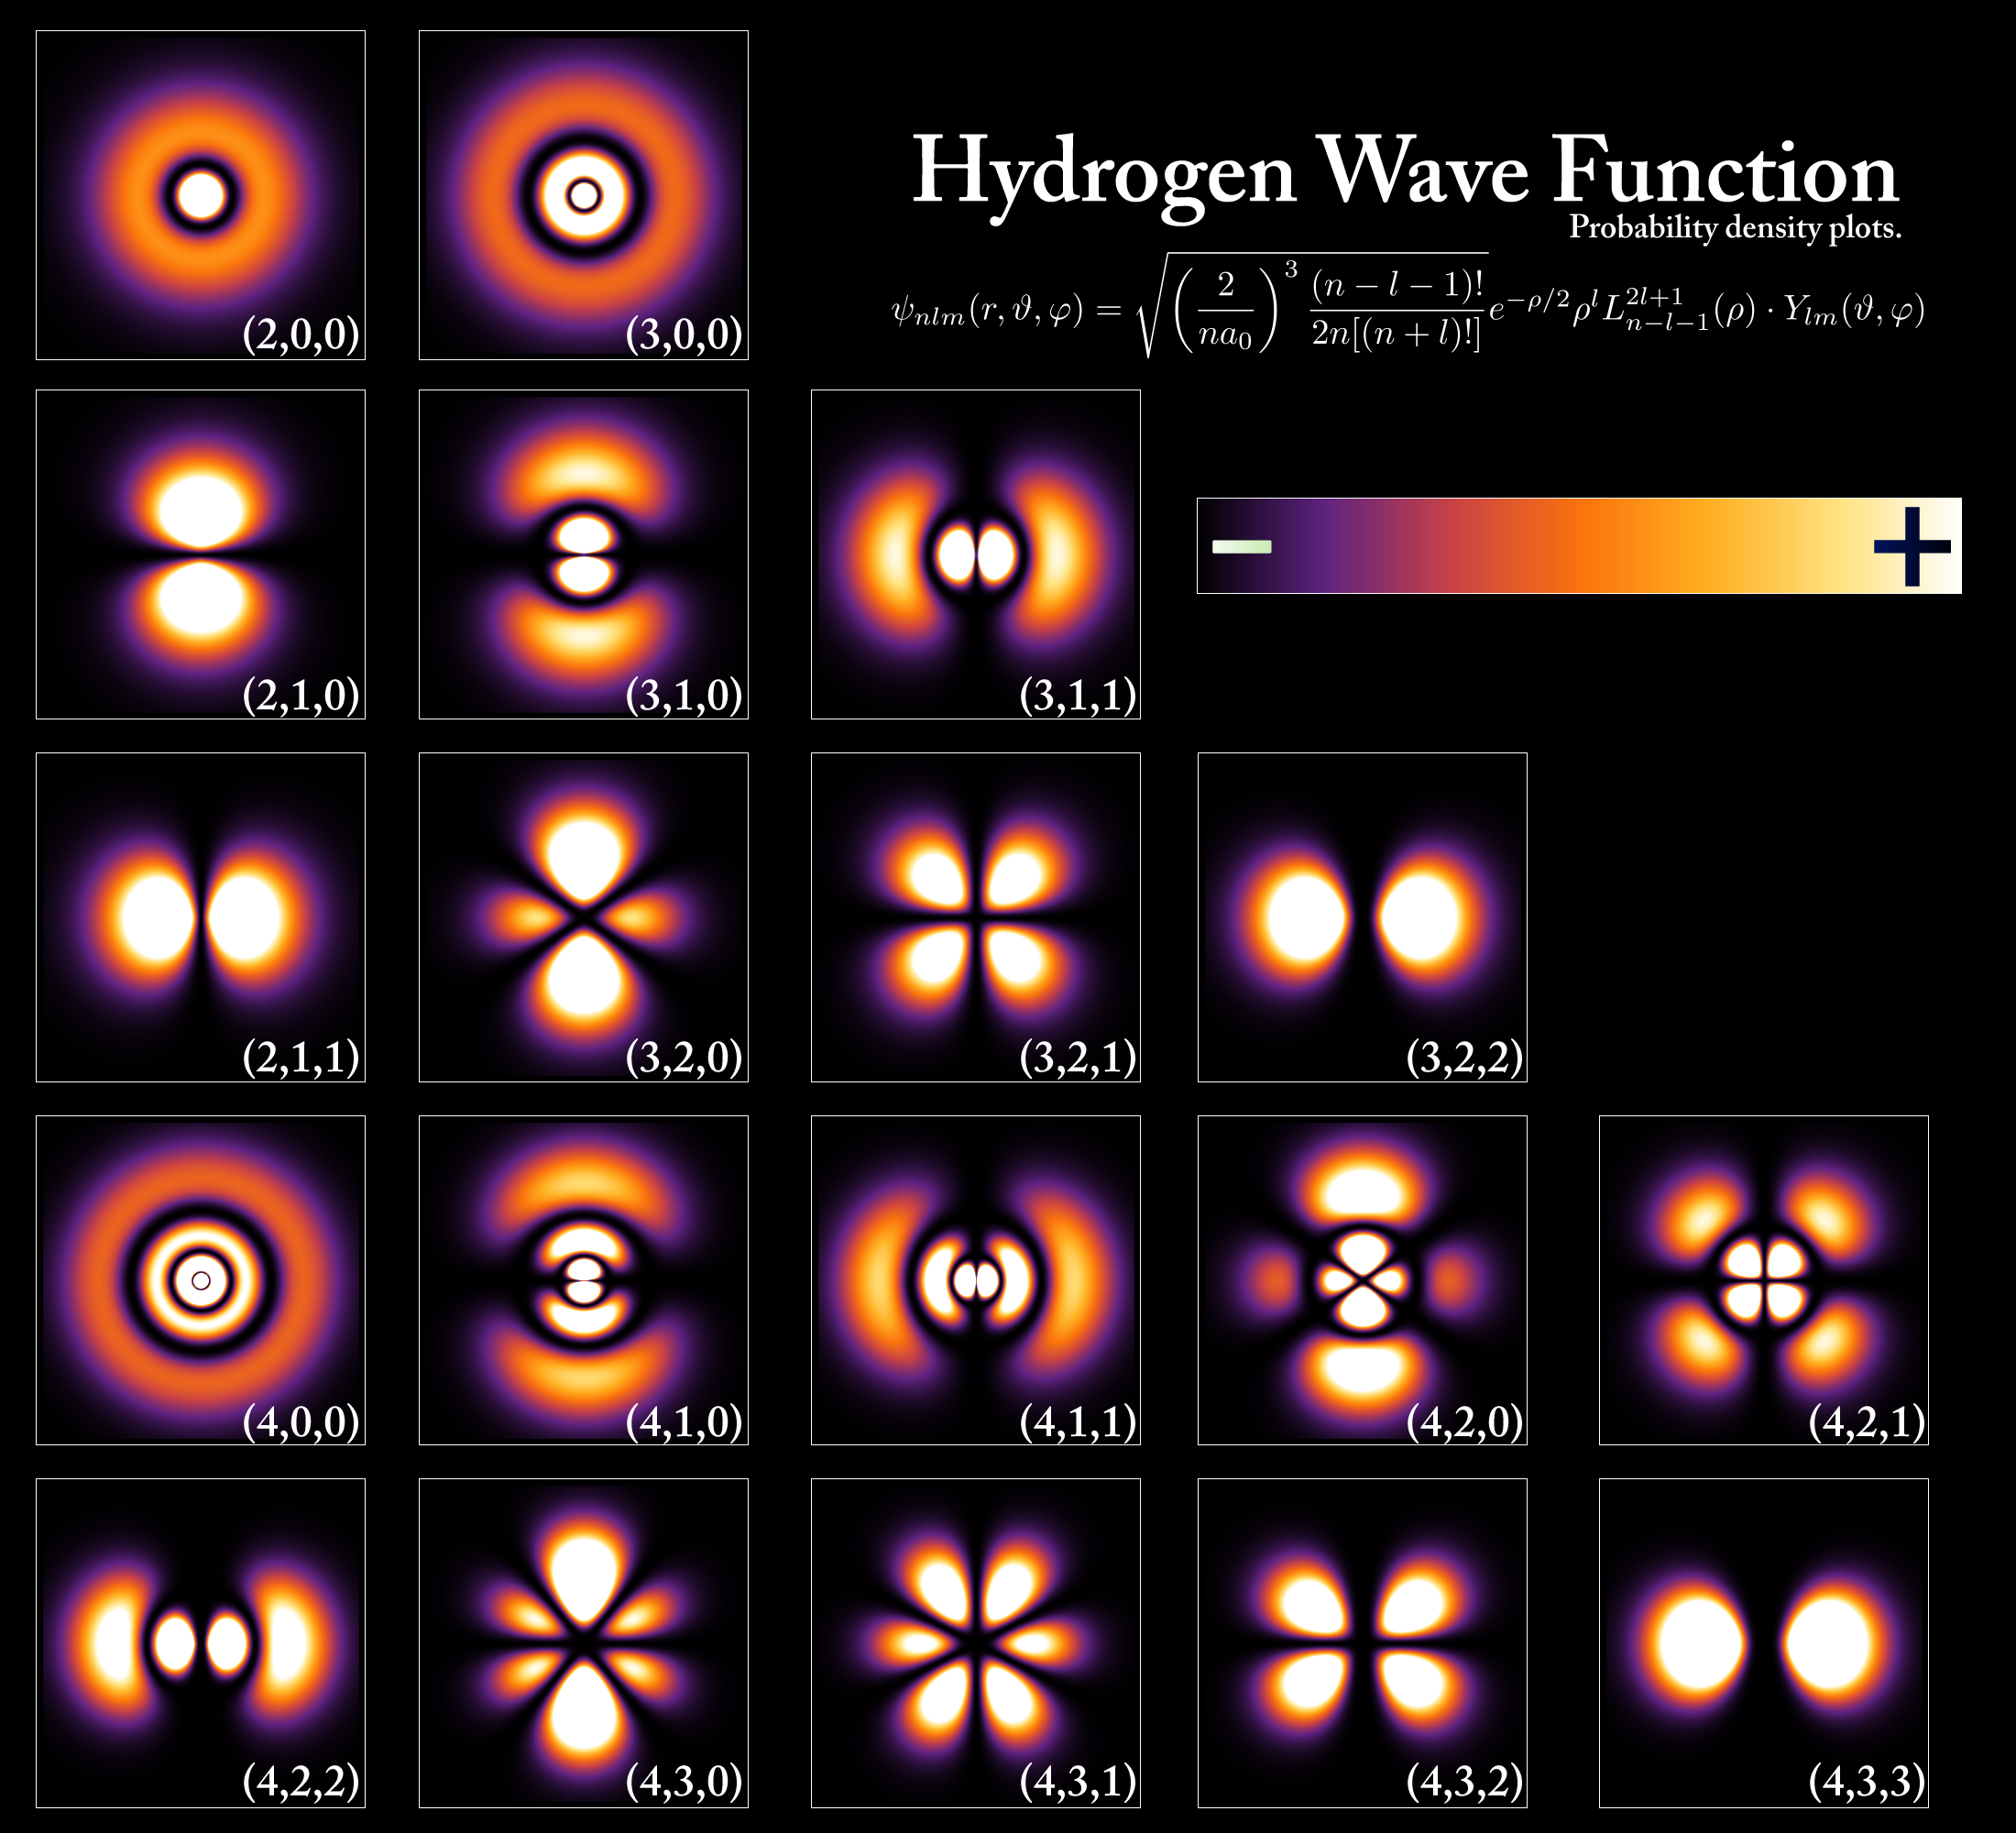
\includegraphics[scale=0.1]{Imagenes/Hydrogen_Density_Plots.png}
    \caption{Gráficas de densidad de estado para el hidrógeno.}
\end{figure}
\end{frame}

\subsection{Espectro del hidrógeno}

\begin{frame}
\frametitle{Modificando el estado}
En principio, si ponemos un átomo de hidrógeno en un estado estacionario $\Psi_{n \ell m}$, debe quedarse allí para siempre.
\end{frame}
\begin{frame}
\frametitle{Modificando el estado}
Sin embargo, si \textocolor{cobalt}{perturbamos} ligeramente (por colisión con otro átomo, por ejemplo, o haciéndole incidir  luz en él), entonces el átomo puede experimentar una transición a otro estado estacionario mediante la absorción de la energía y pasarse a un estado de mayor energía o cediendo energía (normalmente en forma de radiación electromagnética) y moverse  hacia abajo.
\end{frame}
\begin{frame}
\frametitle{Tipos de perturbaciones}
En la práctica este tipo de perturbaciones están siempre presentes; transiciones (o, como a veces se denominan \textocolor{blue}{saltos cuánticos}) se producen constantemente.
\end{frame}
\begin{frame}
\frametitle{Resultado de la perturbación}
El resultado es que un contenedor de hidrógeno emite luz (fotones), cuya energía corresponde a la diferencia de energía entre los estados inicial y final:
\pause
\begin{align}
E_{\gamma} = E_{i} - E_{f} = \SI{-13.6}{\electronvolt} \left( \dfrac{1}{n_{i}^{2}} - \dfrac{1}{n_{f}^{2}} \right)
\label{eq:ecuacion_04_91}
\end{align}
\end{frame}
\begin{frame}
\frametitle{Usando la mecánica cuántica}
De acuerdo con la fórmula de Planck, la energía de un fotón es proporcional a su frecuencia:
\pause
\begin{align}
E_{\gamma} = h \, \nu
\label{eq:ecuacion_04_92}
\end{align}
\end{frame}
\begin{frame}
\frametitle{Usando la mecánica cuántica}
Mientras que la longitud de onda está dada por $\lambda = c / \nu)$, por tanto:
\pause
\begin{align}
\dfrac{1}{\lambda} = R \left( \dfrac{1}{n_{f}^{2}} - \dfrac{1}{n_{i}^{2}} \right)
\label{eq:ecuacion_04_93}
\end{align}
\end{frame}
\begin{frame}
\frametitle{Usando la mecánica cuántica}
Donde:
\pause
\begin{align}
R = \dfrac{m}{4 \, \pi \, c \, \hbar} \left( \dfrac{e^{2}}{4 \, \pi \, \epsilon_{0}} \right)^{2} = \SI{1.097e7}{\per\metre}
\label{eq:ecuacion_04_94}
\end{align}
\pause
a $R$ se le conoce como la \textocolor{darkblue}{constante de Rydberg}, y la ec. (\ref{eq:ecuacion_04_93}) es la \textocolor{darklava}{fórmula Rydberg} para el espectro de hidrógeno.
\end{frame}
\begin{frame}
\frametitle{La fórmula de Rydberg}
Fue descubierto empíricamente en el siglo XIX, y el mayor triunfo de la teoría de Bohr fue su capacidad para dar cuenta de este resultado y calcular $R$ en función de las constantes fundamentales de la naturaleza.
\end{frame}
\begin{frame}
\frametitle{Transiciones en el átomo}
Las transiciones al estado base ($n_{f}= 1$) se encuentran en el ultravioleta; \pause son conocidas por los espectroscopistas como la \textocolor{burgundy}{serie de Lyman}.
\end{frame}
\begin{frame}
\frametitle{Transiciones en el átomo}
Las transiciones al primer estado excitado ($n_{f}= 2$) se encuentran en la zona de región visible; conforman la \textocolor{cadmiumgreen}{serie de Balmer}.
\end{frame}
\begin{frame}
\frametitle{Transiciones en el átomo}
Las transiciones a $n_{f} = 3$ (la \textocolor{cadmiumred}{serie de Paschen}) están en el infrarrojo, y así sucesivamente (véase la figura \ref{fig:figura_espectro_H}).
\end{frame}
\begin{frame}
\frametitle{Transiciones en el átomo}
A temperatura ambiente, la mayoría de los átomos de hidrógeno están en el estado base, para obtener el espectro de emisión, se deben elevar primero los diferentes estados excitados, por lo general esto se realiza haciendo pasar una chispa eléctrica a través del gas.
\end{frame}
\begin{frame}[plain]
\begin{figure}[H]
    \centering
    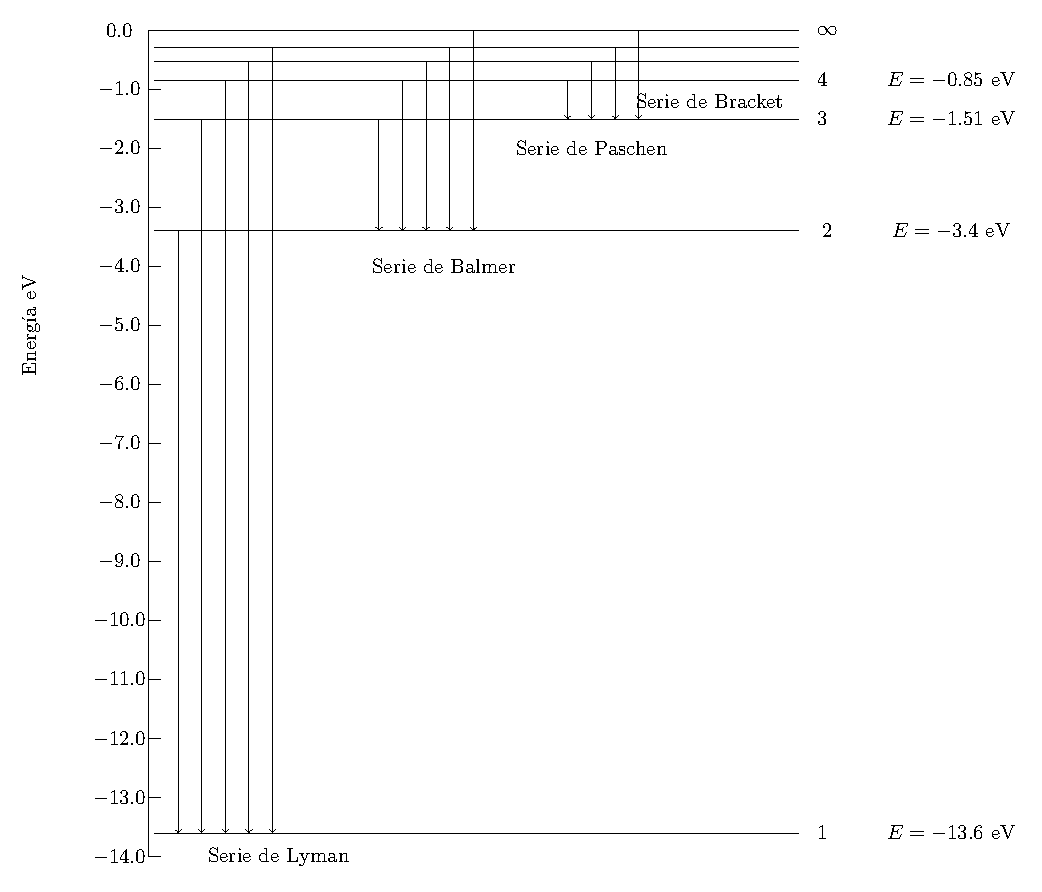
\includegraphics[scale=0.5]{Imagenes/espectrohidrogeno.eps}
    \caption{Niveles de energía y transiciones en el espectro de hidrógeno.}
    \label{fig:figura_espectro_H}
\end{figure}
\end{frame}

\section{Normalización función radial}
\frame[allowframebreaks]{\tableofcontents[currentsection, hideothersubsections]}
\subsection{Marco teórico}

\begin{frame}
\frametitle{Solución completa}
Del estudio de la ecuación del átomo de hidrógeno, se obtuvo la solución general de la ecuación de onda en términos de tres números cuánticos: $n$, $\ell$ y $m$:
\pause
\begin{align*}
\psi_{n \ell m} (r, \theta, \phi) =  R_{n \ell} (r) \, Y_{\ell}^{m} (\theta, \phi)
\end{align*}
\end{frame}
\begin{frame}
\frametitle{Solución parte radial}
Donde la parte radial a la solución está dada por:
\pause
\begin{align*}
R_{n \ell}(r) = \dfrac{1}{r} \, \rho^{\ell + 1} \, e^{-\rho} \, v(\rho)
\end{align*}
\\
\bigskip
\pause
En particular para $R_{20}$, se tiene que:
\pause
\begin{align*}
R_{20}(r) = \dfrac{c_{0}}{2 \, a} \left( 1 - \dfrac{r}{2 \, a} \right) \, e^{-r/2a}
\end{align*}
\end{frame}

%Ref. Griffits (2005) Problem 4.11 (a)
\subsection{Ejercicio 1}

\begin{frame}
\frametitle{Enunciado del problema}
Normaliza la función $R_{20}$ para construir la función $\psi_{200}$.
\\
\bigskip
\pause
¿Qué tenemos que hacer? \pause
De la función:
\pause
\begin{align*}
R_{20}(r) = \dfrac{c_{0}}{2 \, a} \left( 1 - \dfrac{r}{2 \, a} \right) \, e^{-r/2a}
\end{align*}
Hay que determinar los coeficientes $c_{0}$.
\end{frame}

\subsection*{Solución}

\begin{frame}
\frametitle{Punto de partida}
Partimos de la normalización de la función:
\pause
\begin{align*}
\scaleint{6ex}_{\bs 0}^{\infty} \abs{R_{20}}^{2} \, r^{2} \dd{r} = 1
\end{align*}
\pause
Por lo que:
\pause
\begin{align*}
\scaleint{6ex}_{\bs 0}^{\infty} \abs{ \dfrac{c_{0}}{2 \, a} \left( 1 - \dfrac{r}{2 \, a} \right) \, e^{-r/2a} }^{2} r^{2} \dd{r} = 1
\end{align*}
\end{frame}
\begin{frame}
\frametitle{Desarrollo}
Entonces tenemos que:
\pause
\begin{align*}
\scaleint{6ex}_{\bs 0}^{\infty} \left(\dfrac{c_{0}}{2 \, a}\right)^{2} \left( 1 - \dfrac{r}{2 \, a} \right)^{2} \, e^{-r/a} \, r^{2} \dd{r} = 1
\end{align*}
\\
\bigskip
\pause
Para resolver esta integral, \pause proponemos el cambio de variable: $z = \dfrac{r}{a}$
\end{frame}
\begin{frame}
\frametitle{Expresión con el cambio}
\begin{align*}
\scaleint{6ex}_{\bs 0}^{\infty} \bigg( \dfrac{c_{0}}{2 \, a} \bigg)^{2} \, \bigg( 1 - \dfrac{z}{2} \bigg)^{2} \, e^{-z} \, (a \, z)^{2} a \, \dd{z} = 1
\end{align*}
\\
\bigskip
\pause
Que simplificando, obtenemos:
\pause
\begin{align*}
\bigg( \dfrac{c_{0}}{2 \, a} \bigg)^{2} \, a^{3} \, \scaleint{6ex}_{\bs 0}^{\infty} \bigg( 1 - \dfrac{z}{2} \bigg)^{2} \, e^{-z} \, z^{2} \dd{z} = 1
\end{align*}
\end{frame}
\begin{frame}
\frametitle{Resolviendo la integral}
Desarrollando el binomio en el integrando:
\pause
\begin{align*}
\dfrac{c_{0}^{2} \, a}{4} \, \scaleint{6ex}_{\bs 0}^{\infty} \left( 1 - z + \dfrac{z^{2}}{4} \right) \, e^{-z} \, z^{2} \dd{z} = 1
\end{align*}
\pause
Entonces tendremos:
\pause
\begin{align*}
\dfrac{c_{0}^{2} \, a}{4} \, \scaleint{6ex}_{\bs 0}^{\infty} \left( z^{2} - z^{3} + \dfrac{z^{2}}{4} \right) \, e^{-z} \dd{z} = 1
\end{align*}
\end{frame}
\begin{frame}
\frametitle{Ocupando un resultado conocido}
Sabemos que una integral del tipo:
\pause
\begin{eqnarray*}
\scaleint{6ex}_{\bs 0}^{\infty} z^{n} \, e^{-z} \dd{z} = \pause \Gamma(n + 1) = \pause n!
\end{eqnarray*}
\pause
Por lo que la integral anterior se resuelve en términos del valor del factorial de cada término:
\end{frame}
\begin{frame}
\frametitle{Solución a la integral}
Al resolver la integral de la suma de cada término, tendremos que:
\pause
\begin{equation*}
\begin{aligned}
\dfrac{c_{0}^{2} \, a}{4} \, &\left[ 2 - 6 + \dfrac{24}{4} \right] = 1 \\[0.5em] \pause
\dfrac{a}{2} \, c_{0}^{2} &= 1 \\[0.5em] \pause
\Rightarrow c_{0} &= \sqrt{\dfrac{2}{a}}
\end{aligned}
\end{equation*}
\end{frame}
\begin{frame}
\frametitle{La función radial ya es conocida}
Una vez obtenido el valor de $c_{0}$ ya se puede ocupar para la función radial:
\pause
\begin{align*}
R_{20} (r) = \sqrt{\dfrac{2}{a}} \, \dfrac{1}{2 a} \bigg( 1 - \dfrac{r}{2 a} \bigg) \, e^{-r/2a}
\end{align*}
\end{frame}
\begin{frame}
\frametitle{Gráfica de la función radial}
\begin{figure}
   \centering
   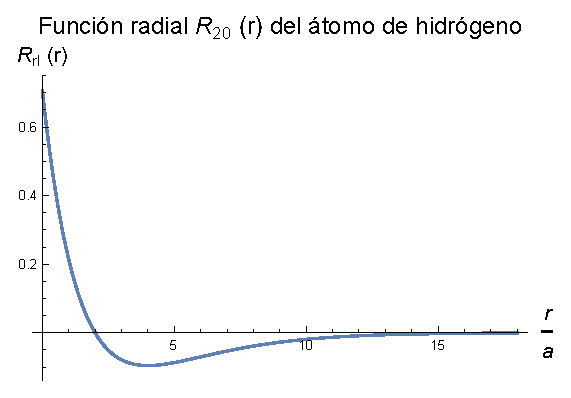
\includegraphics[scale=1]{Imagenes/Plot_Hermite_Radial_20.eps}
\end{figure}
\end{frame}
\begin{frame}
\frametitle{La solución}
La solución general es:
\pause
\begin{align*}
\psi_{n \ell m} (r, \theta, \phi) = R_{n \ell} (r) \, Y_{\ell}^{m} \, (\theta, \phi)
\end{align*}
\pause
Lo que nos pide el enunciado es:
\pause
\begin{align*}
\psi_{200} = R_{2 0} (r) \, Y_{0}^{0} \, (\theta, \phi)
\end{align*}
\end{frame}
\begin{frame}
\frametitle{Otro resultado conocido}
Como ya conocemos el valor del armónico esférico:
\pause
\begin{align*}
Y_{0}^{0} \, (\theta, \phi) = \dfrac{1}{\sqrt{4 \, \pi}}
\end{align*}
\end{frame}
\begin{frame}
\frametitle{Solución al problema}
Juntamos los resultados, para llegar a:
\pause
\begin{eqnarray*}
\begin{aligned}
\psi_{200} &= \dfrac{1}{\sqrt{4 \, \pi}} \, \sqrt{\dfrac{2}{a}} \, \dfrac{1}{2 \, a} \bigg( 1 - \dfrac{r}{2 \, a} \bigg) \, e^{-r/2a} \\[1em] \pause
\psi_{200} &= \dfrac{1}{\sqrt{2 \, \pi \, a}} \, \dfrac{1}{2 \, a} \bigg( 1 - \dfrac{r}{2 \, a} \bigg) \, e^{-r/2a} \qed
\end{aligned}
\end{eqnarray*}
\end{frame}
\begin{frame}
\frametitle{Gráfica en 3D}
Una visualización de la función de onda $\psi_{200}$ se muestra a continuación:
\end{frame}
\begin{frame}[plain]
\begin{figure}
    \centering
    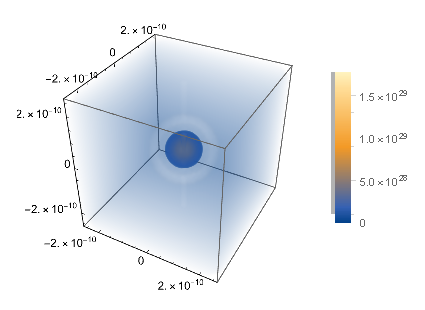
\includegraphics[scale=1]{Imagenes/Plot_Funcion_Onda_200.eps}
\end{figure}
\end{frame}

%Ref. Griffits (2005) Problem 4.11 (b)
\subsection{Ejercicio 2}

\begin{frame}
\frametitle{Enunciado del ejercicio}
Normaliza la función radial:
\pause
\begin{align*}
R_{21} (r) = \dfrac{c_{0}}{4 a^{2}} \, r \, e^{-r/2a}
\end{align*}
\pause
Para construir las funciones de onda: $\psi_{211}, \psi_{210}$ y $\psi_{21-1}$
\end{frame}
\begin{frame}
\frametitle{Nuevamente la normalización}
Para obtener el valor del coeficiente $c_{0}$, debemos de normalizar la función $R_{21} (r)$:
\pause
\begin{align*}
\scaleint{6ex}_{\bs 0}^{\infty} \abs{R_{21}}^{2} \, r^{2} \, \dd{r} = 1
\end{align*}
\end{frame}
\begin{frame}
\frametitle{Expresión a calcular}
Entonces se tiene que:
\pause
\begin{eqnarray*}
\begin{aligned}
&\scaleint{6ex}_{\bs 0}^{\infty} \bigg( \dfrac{c_{0}}{4 a^{2}} \, r \, e^{-r/2a} \bigg)^{2} \, r^{2} \dd{r} = 1 \\[0.5em] \pause
&\dfrac{c_{0}^{2}}{16 a^{4}} \, \scaleint{6ex}_{\bs 0}^{\infty}  r^{4} \, e^{-r/a} \dd{r} = 1
\end{aligned}
\end{eqnarray*}
\end{frame}
\begin{frame}
\frametitle{Hacemos cambio de variable}
Se ocupa el mismo cambio de variable que en el ejercicio anterior, es decir: $z = r/a$:
\pause
\begin{eqnarray*}
\begin{aligned}
&\dfrac{c_{0}^{2} \, a}{16} \, \scaleint{6ex}_{\bs 0}^{\infty}  z^{4} \, e^{-z} \dd{z} = 1 \\[0.5em] \pause
\Rightarrow \hspace{0.2cm} &\dfrac{c_{0}^{2} \, a}{16} \, (4!) = 1 \\[0.5em] \pause
\Rightarrow \hspace{0.2cm} &\dfrac{3 \, c_{0}^{2} \, a}{2} = 1 \pause \hspace{0.5cm} \Rightarrow \hspace{0.2cm} c_{0} = \sqrt{\dfrac{2}{3 \, a}}
\end{aligned}
\end{eqnarray*}
\end{frame}
\begin{frame}
\frametitle{La función radial}
Por lo que la función radial $R_{21} (r)$ es:
\pause
\begin{align*}
R_{21} (r) = \dfrac{1}{\sqrt{6 \, a}} \, \dfrac{1}{2 \, a^{2}} \, r \, e^{-2/ra}
\end{align*}
\end{frame}
\begin{frame}
\frametitle{Gráfica de la función radial}
\begin{figure}
   \centering
   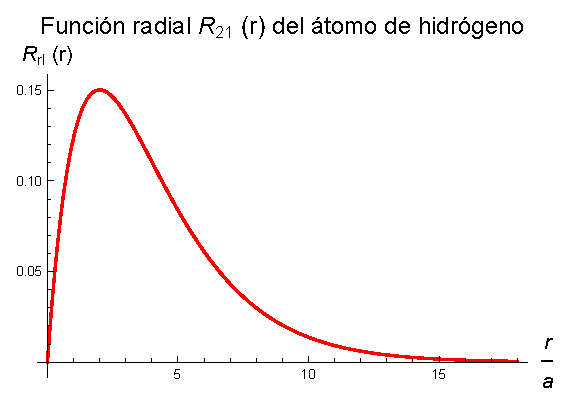
\includegraphics[scale=1]{Imagenes/Plot_Hermite_Radial_21.eps}
\end{figure}
\end{frame}
\begin{frame}
\frametitle{Ocupando los armónicos esféricos}
Para la solución completa, debemos de ocupar los armónicos esféricos:
\pause
\begin{align*}
Y_{1}^{0} (\theta, \phi) = \bigg( \dfrac{3}{4 \, \pi} \bigg)^{\frac{1}{2}} \cos \theta
\end{align*}
\pause
De manera conveniente, tenemos que:
\pause
\begin{align*}
Y_{1}^{\pm 1} (\theta, \phi) = \mp \bigg( \dfrac{3}{8 \, \pi} \bigg)^{\frac{1}{2}} \sin \theta \, e^{\pm i \phi}
\end{align*}
\end{frame}
\begin{frame}
\frametitle{Solución para $\psi_{210}$}
Al juntar los resultados de la parte radial y el correspondiente armónico esférico, la solución es:
\pause
\begin{eqnarray*}
\begin{aligned}
\psi_{210} (r, \theta, \phi) &= \dfrac{1}{\sqrt{6 \, a}} \, \dfrac{1}{2 \, a^{2}} \, r \, e^{-r/2a} \, \sqrt{\dfrac{3}{4 \, \pi}} \cos \theta = \\[0.5em] \pause
&= \dfrac{1}{2 \, \pi \, a} \, \dfrac{1}{4 \, a^{2}} \, r \, e^{-r/2a} \, \cos \theta
\end{aligned}
\end{eqnarray*}
\end{frame}
\begin{frame}
\frametitle{Solución para $\psi_{21 \pm 1}$}
Al juntar ahora los resultados de la parte radial y el correspondiente armónico esférico, cuidando los signos, la solución es:
\pause
\begin{eqnarray*}
\begin{aligned}
\psi_{21 \pm 1} (r, \theta, \phi) &= \dfrac{1}{\sqrt{6 \, a}} \, \dfrac{1}{2 \, a^{2}} \, r \, e^{-r/2a} \times \\[0.5em]
&\times \bigg[ \mp \, \sqrt{\dfrac{3}{8 \, \pi}} \, \sin \theta \, e^{\pm i \phi} \bigg]  =
\end{aligned}
\end{eqnarray*}
\end{frame}
\begin{frame}
\frametitle{Solución para $\psi_{21 \pm 1}$}
La solución simplificada para las funciones radiales es:
\pause
\begin{align*}
\psi_{21 \pm 1} (r, \theta, \phi) = \mp \, \dfrac{1}{\sqrt{\pi \, a}} \, \dfrac{1}{8 \, a^{2}} \, r \, e^{-2/ra} \, \sin \theta \, e^{\pm i \phi}
\end{align*}
\end{frame}
\begin{frame}
\frametitle{Gráfica en 3D}
Una visualización de la función de onda $\psi_{21 \pm 1}$ se muestra a continuación:
\pause
\begin{figure}
   \centering
   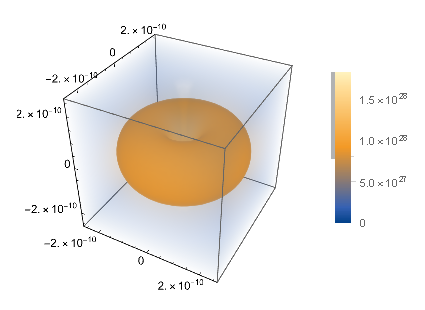
\includegraphics[scale=1]{Imagenes/Plot_Funcion_Onda_211.eps}
\end{figure}
\end{frame}

\end{document}